%*************************************************
% In this file the first few pages are typeset.
% Make changes accordingly.
%*************************************************

% شماره صفحات با حروف
\pagenumbering{adadi}

%***************************
% Page 1: Besmelah
%***************************
\thispagestyle{empty}
\begin{center}
	~\vfill
	
\includegraphics[scale=1]{besm.jpg}
	~\vfill
\end{center}
\pagebreak

%***************************
% Page 2: Title
%***************************
\thispagestyle{empty}
\newgeometry{left=3cm,right=3cm,top=2cm}
\begin{center}
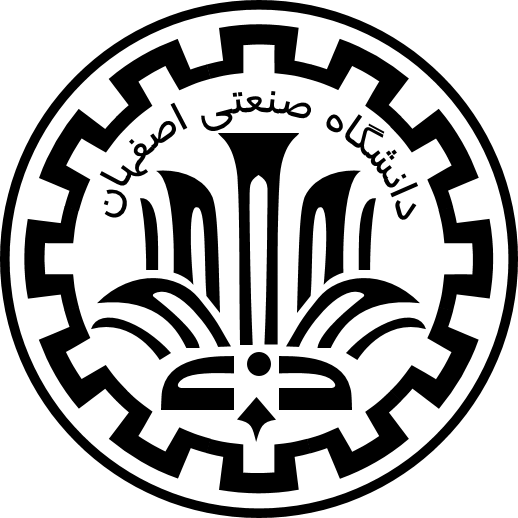
\includegraphics[height=3cm]{iut_logo.png}
\vspace{0.4cm}

{\large
	\textbf{دانشگاه صنعتی اصفهان}\\
	دانشکده مهندسی برق و کامپیوتر
}
\vspace{3.5cm}

{\LARGE
	\textbf{
	بهبود کارایی الگوریتم یادگیری فدرال برای داده‌های غیرمستقل و غیریکنواخت با در نظر گرفتن میزان شباهت بین شبکه‌های عصبی در دستگاه‌های نهایی
	}
	\\
}
\vspace{3.5cm}

{\large
	\textbf{پایان‌نامه کارشناسی ارشد مهندسی کامپیوتر - هوش مصنوعی و رباتیکز}
}
\vspace{1cm}

{\Large
	\textbf{علی بزرگ‌زاد}\\
}
\vspace{2.5cm}

{\large
	استادراهنما\\
}
\vspace{0.5cm}

{\Large
	\textbf{دکتر امیر خورسندی}\\
}
\vspace{3.5cm}

{\Large
	\textbf{1403}
}

\end{center}
\restoregeometry
\pagebreak




%***************************
% Page3: Acknowledgment (Optional)
%***************************
%\thispagestyle{empty}
%\vspace*{3cm}
%
%{\large
%	\textbf{تشکر و قدردانی}\\
%
%	
%پروردگار منّان را سپاسگزارم ......
%
%}
%\restoregeometry
%\pagebreak


%***************************
% Page4: Rules
%***************************
\thispagestyle{empty}
\vspace*{3cm}

{\large
	\doublespacing
		\textbf{
		کلیه حقوق مالکیت مادی و معنوی مربوط به اين پايان نامه متعلق به دانشگاه صنعتی اصفهان و پدیدآورندگان است. این حقوق توسط دانشگاه صنعتي اصفهان و بر اساس خط مشی مالکیت فکری این دانشگاه، ارزش‌گذاری و سهم بندي خواهد شد. هر گونه بهره برداري از محتوا، نتايج یا اقدام براي تجاري‌سازي دستاوردهاي اين پايان نامه تنها با مجوز کتبی دانشگاه صنعتی اصفهان امکان‌پذیر است.
		}\\
	}
\restoregeometry
\pagebreak


%***************************
% 8th page: Table of contents
%***************************

\titleformat{\chapter}[display]
	{\normalfont\LARGE\bfseries\centering}{\chaptertitlename ~ \tartibi{chapter}}{20pt}{\LARGE}
\newgeometry{left=2.5cm,right=3cm,top=3cm,bottom=2.5cm,includehead=false,headsep=1cm,footnotesep=.5cm}
\baselineskip=.7cm

\addtocontents{toc}{\textbf{\underline{عنوان}}}
\addtocontents{toc}{\hfill\textbf{\underline{صفحه}}\par}
\addcontentsline{toc}{section}{فهرست مطالب}
\tableofcontents
\pagebreak


%\renewcommand\listfigurename{فهرست شکل‌ها}
%\addcontentsline{toc}{section}{فهرست شکل‌ها}
%\listoffigures
%\pagebreak

% change the font and margins of a chapter title
\titlespacing*{\chapter}{0pt}{3.5cm}{6cm}
\titleformat{\chapter}[display]
	{\normalfont\LARGE\bfseries\raggedright}{\chaptertitlename ~ \tartibi{chapter}}{20pt}{\LARGE}

% No page numbers on the first page of a chapter
\assignpagestyle{\chapter}{empty}
